\documentclass[11pt, a4paper, twoside, titlepage]{article}
\usepackage[utf8]{inputenc}
\usepackage[a4paper]{geometry}
\usepackage{french}
\usepackage{graphicx}
\usepackage{caption}

\geometry{hscale=0.75,vscale=0.75,centering}
\font\titlefont=cmr12 at 21pt
\graphicspath{ {images/} }

\begin{document}


\title{{\titlefont Projet d'architecture matérielle}\\ARMAgeddon\thanks{J'aime les jeux de mots}}
\author{Pierre KOEBELIN}
\date{\today} 
\maketitle


\begin{abstract}

	L’objectif de ce projet était la réalisation d’un mini-processeur dans Diglog. Pour ce faire, nous devions nous appuyer sur le jeu d'instructions d'un processeur MIPS, que nous avons implémenté dans le logiciel Diglog\ldots\\
\\

\end{abstract}

\tableofcontents

\newpage
\section{ALU}
	Cet ALU permet de faire de nombreuses opérations sur des entiers sur 8 bits, comme l'addition et la soustraction en signée et non signée, ainsi que le complément à 1, l'incrémentation, l'opposé et les ET et OU binaires.\\
	\begin{center}
		\centerline{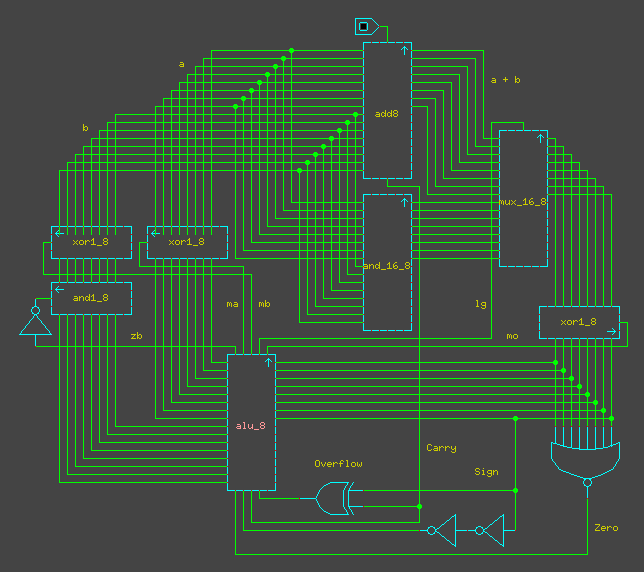
\includegraphics[width=0.8\textwidth]{alu_8}}
		\captionof{figure}{ALU à 5 bits de contrôle et 4 bits de sortie}
	\end{center}
	Pour ce faire, il prend en entrée deux entiers codés sur 8 bits et est géré par 5 bits de contrôle.\\
	Il propose en sortie le résultat de l'opération sur 8 bits, ainsi que 4 bits de sortie: \texttt{Zero}, \texttt{Sign}, \texttt{Carry} et \texttt{Overflow}.

\newpage
\subsection{Bits de contrôle}
	Ces bits de contrôle permettent de réaliser différentes opérations sur les entrées \texttt{a} et \texttt{b}.\\
	\\
	\centerline{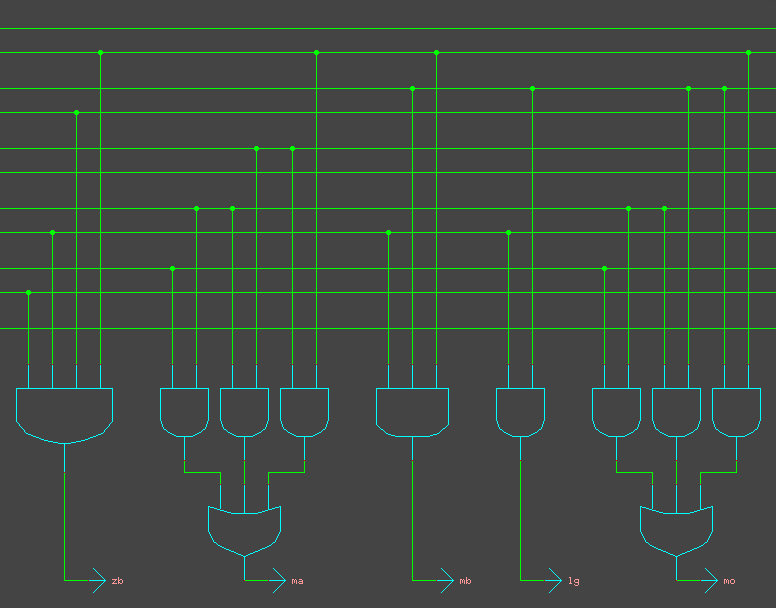
\includegraphics[width=0.8 \textwidth]{log_alu}}
	\captionof{figure}{Calcul des bits de contrôle de l'ALU}

\subsubsection{zb}
	Ce bit de contrôle gère le bloc \texttt{and1\_8} situé sur les bits de \texttt{b}, et permet de mettre \texttt{b} à 0 ou non avant de passer par le bloc \texttt{xor1\_8}.

\subsubsection{ma}
	Ce bit de contrôle gère le bloc \texttt{xor1\_8} situé sur les bits de \texttt{a}, et permet de donner son complément à 1 avant d'être utilisé par \texttt{add8} et \texttt{and\_16\_8}.

\subsubsection{mb}
	Ce bit de contrôle gère le bloc \texttt{xor1\_8} situé sur les bits de \texttt{b}, et permet de donner son complément à 1 avant d'être utilisé par \texttt{add8} et \texttt{and\_16\_8}.

\subsubsection{lg}
	Ce bit de contrôle gère le multiplexeur \texttt{mux\_16\_8} permettant de retourner le résultat de \texttt{add8} ou celui de \texttt{and\_16\_8}.

\subsubsection{mo}
	Ce bit de contrôle gère le bloc \texttt{xor1\_8} situé après le multiplexeur \texttt{mux\_16\_8}, et permet retourner le résultat de \texttt{add8} et \texttt{and\_16\_8} ou son complément à 1.

\subsection{Bits de sortie}

\subsubsection{\texttt{Zero}}
	Ce bit de sortie est à 1 lorsque le résultat de l'opération est nul. Dans le cas d'une soustraction, il indique donc une égalité.

\subsubsection{\texttt{Sign}}
	Ce bit de sortie est identique au bit de poids le plus fort dans le résultat de l'opération, et indique son signe dans le cas d'un entier signé.

\subsubsection{\texttt{Carry}}
	Ce bit de sortie est la retenue en sortie du bloc \texttt{add\_8}.
\subsubsection{\texttt{Overflow}}
	Ce bit indique qu'il y a eu un Overflow.

\section{Modifications apportées au processeur}

\subsection{Implémentation des prédicats}
	Les instruction de type \texttt{1a} possèdent 2 bits actuellement inutilisés. Il est donc possible d'y attribuer dse valeurs afin de modifier ces instructions.\\
	Le but ici est d'autoriser leur réalisation durant l'exécution selon le résultat de la comparaison de deux valeurs.
	\begin{center}
		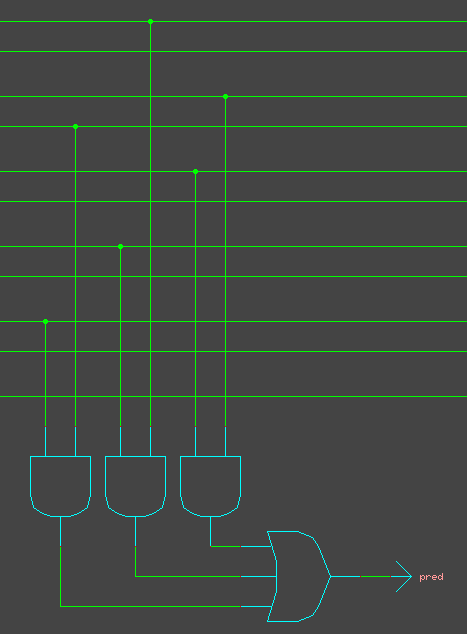
\includegraphics[width=0.5 \textwidth]{log_pred}
		\captionof{figure}{Calcul des bits de contrôle de l'ALU}
	\end{center}

\subsection{Introduction du registre \texttt{flags} et gestion des prédicats}
	\begin{center}
		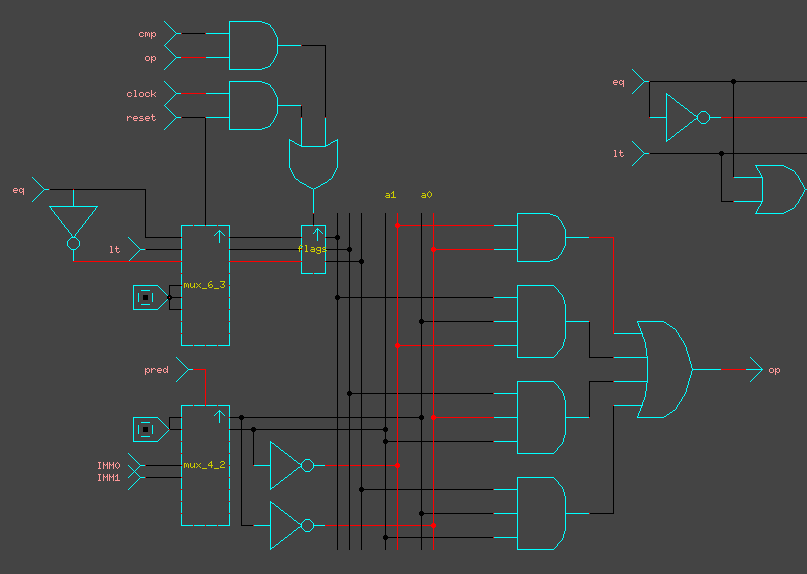
\includegraphics[width=0.8 \textwidth]{mgr_cmp}
		\captionof{figure}{Calcul des bits de contrôle de l'ALU}
	\end{center}

\newpage
\section{Modifications apportées au compilateur}

\subsection{Gestion des prédicats}

\newpage
\section{Codes de tests}

\end{document}